% \chapter{Case Studies}

% %============================= INTRODUCTION =================================
% \section{Introduction}\label{sec:i}
% Remember that wherever you want you can cite with \verb.\cite{a1}. \cite{a1}, \cite{b1} and/or \cite{m1} someone.
% Or use \verb.\footnote{That's a footnote}. like this\footnote{That's a footnote} 
% % this is used to include other .tex files in order to split a long document 

% %============================= SECTIONS =================================
% \section{Selection of Case Studies}

% Justification for the selection of specific narratives is provided, ensuring they offer diverse and rich geospatial content. Background information on each narrative sets the context for their analysis.

% \section{Application of the Ontology}

% This section describes how the ontology is applied to the selected narratives. It discusses the process of annotating the texts and mapping narrative elements to the ontology, highlighting any challenges faced.

% \section{Results and Findings}

% The outcomes of the case studies are presented, including the geospatial knowledge extracted and any patterns observed. Visualizations such as maps or graphs may be used to illustrate the findings.
\chapter{A Semantic-Web Framework to Represents Geospatial Knowledge in Narratives}\label{chap:SW-framework}

\section{Introduction}\label{VI-sec:introduction}

The framework designed to validate and evaluate the NOnt+S ontology is a comprehensive Semantic Web-based system. It is engineered to construct, enhance, and manage a geospatial knowledge graph that supports advanced reasoning and querying. This framework is designed with modular components that allow for seamless integration of datasets, geospatial enrichment, reasoning, and visualization. The following chapter outlines the structure and functionality of this framework, highlighting its key modules and their interactions.

The NOnt+S ontology was applied to real-world case studies from the \acrshort{MOVINGLabel}\cite{MOVINGHorizon2020} and \acrshort{IMAGOLabel}\cite{IMAGOProject} projects, each offering distinct datasets and challenges and will be presented in next chapters. Through its architecture, the framework ensures that geospatial narratives are not only represented semantically but are also enhanced with advanced capabilities for reasoning and querying. Below, the main components of the architecture are described in detail, focusing on their individual roles and how they work together to process and analyze geospatial data.

The architecture of the NOnt+S framework is designed to facilitate the entire data lifecycle, from ingestion to analysis. The central objective is to build a \textit{knowledge graph}—a structured representation of geospatial information, enriched with semantic annotations that allow for more sophisticated data interactions. The key features of the framework are displayed in  \Cref{fig:SemanticFramework}:
\begin{itemize}
    \item \textit{Linking and Enhancement} from diverse sources,
    \item \textit{Semantic representation} using the NOnt+S ontology,
    \item \textit{Knowledge graph construction},
    \item \textit{Reasoning} capabilities for generating new knowledge,
    \item \textit{Triplestore-based storage} for efficient data retrieval and management,
    \item \textit{Advanced querying} and visualization of geospatial data.
\end{itemize}

\begin{figure}[h!tb]
    \centerline {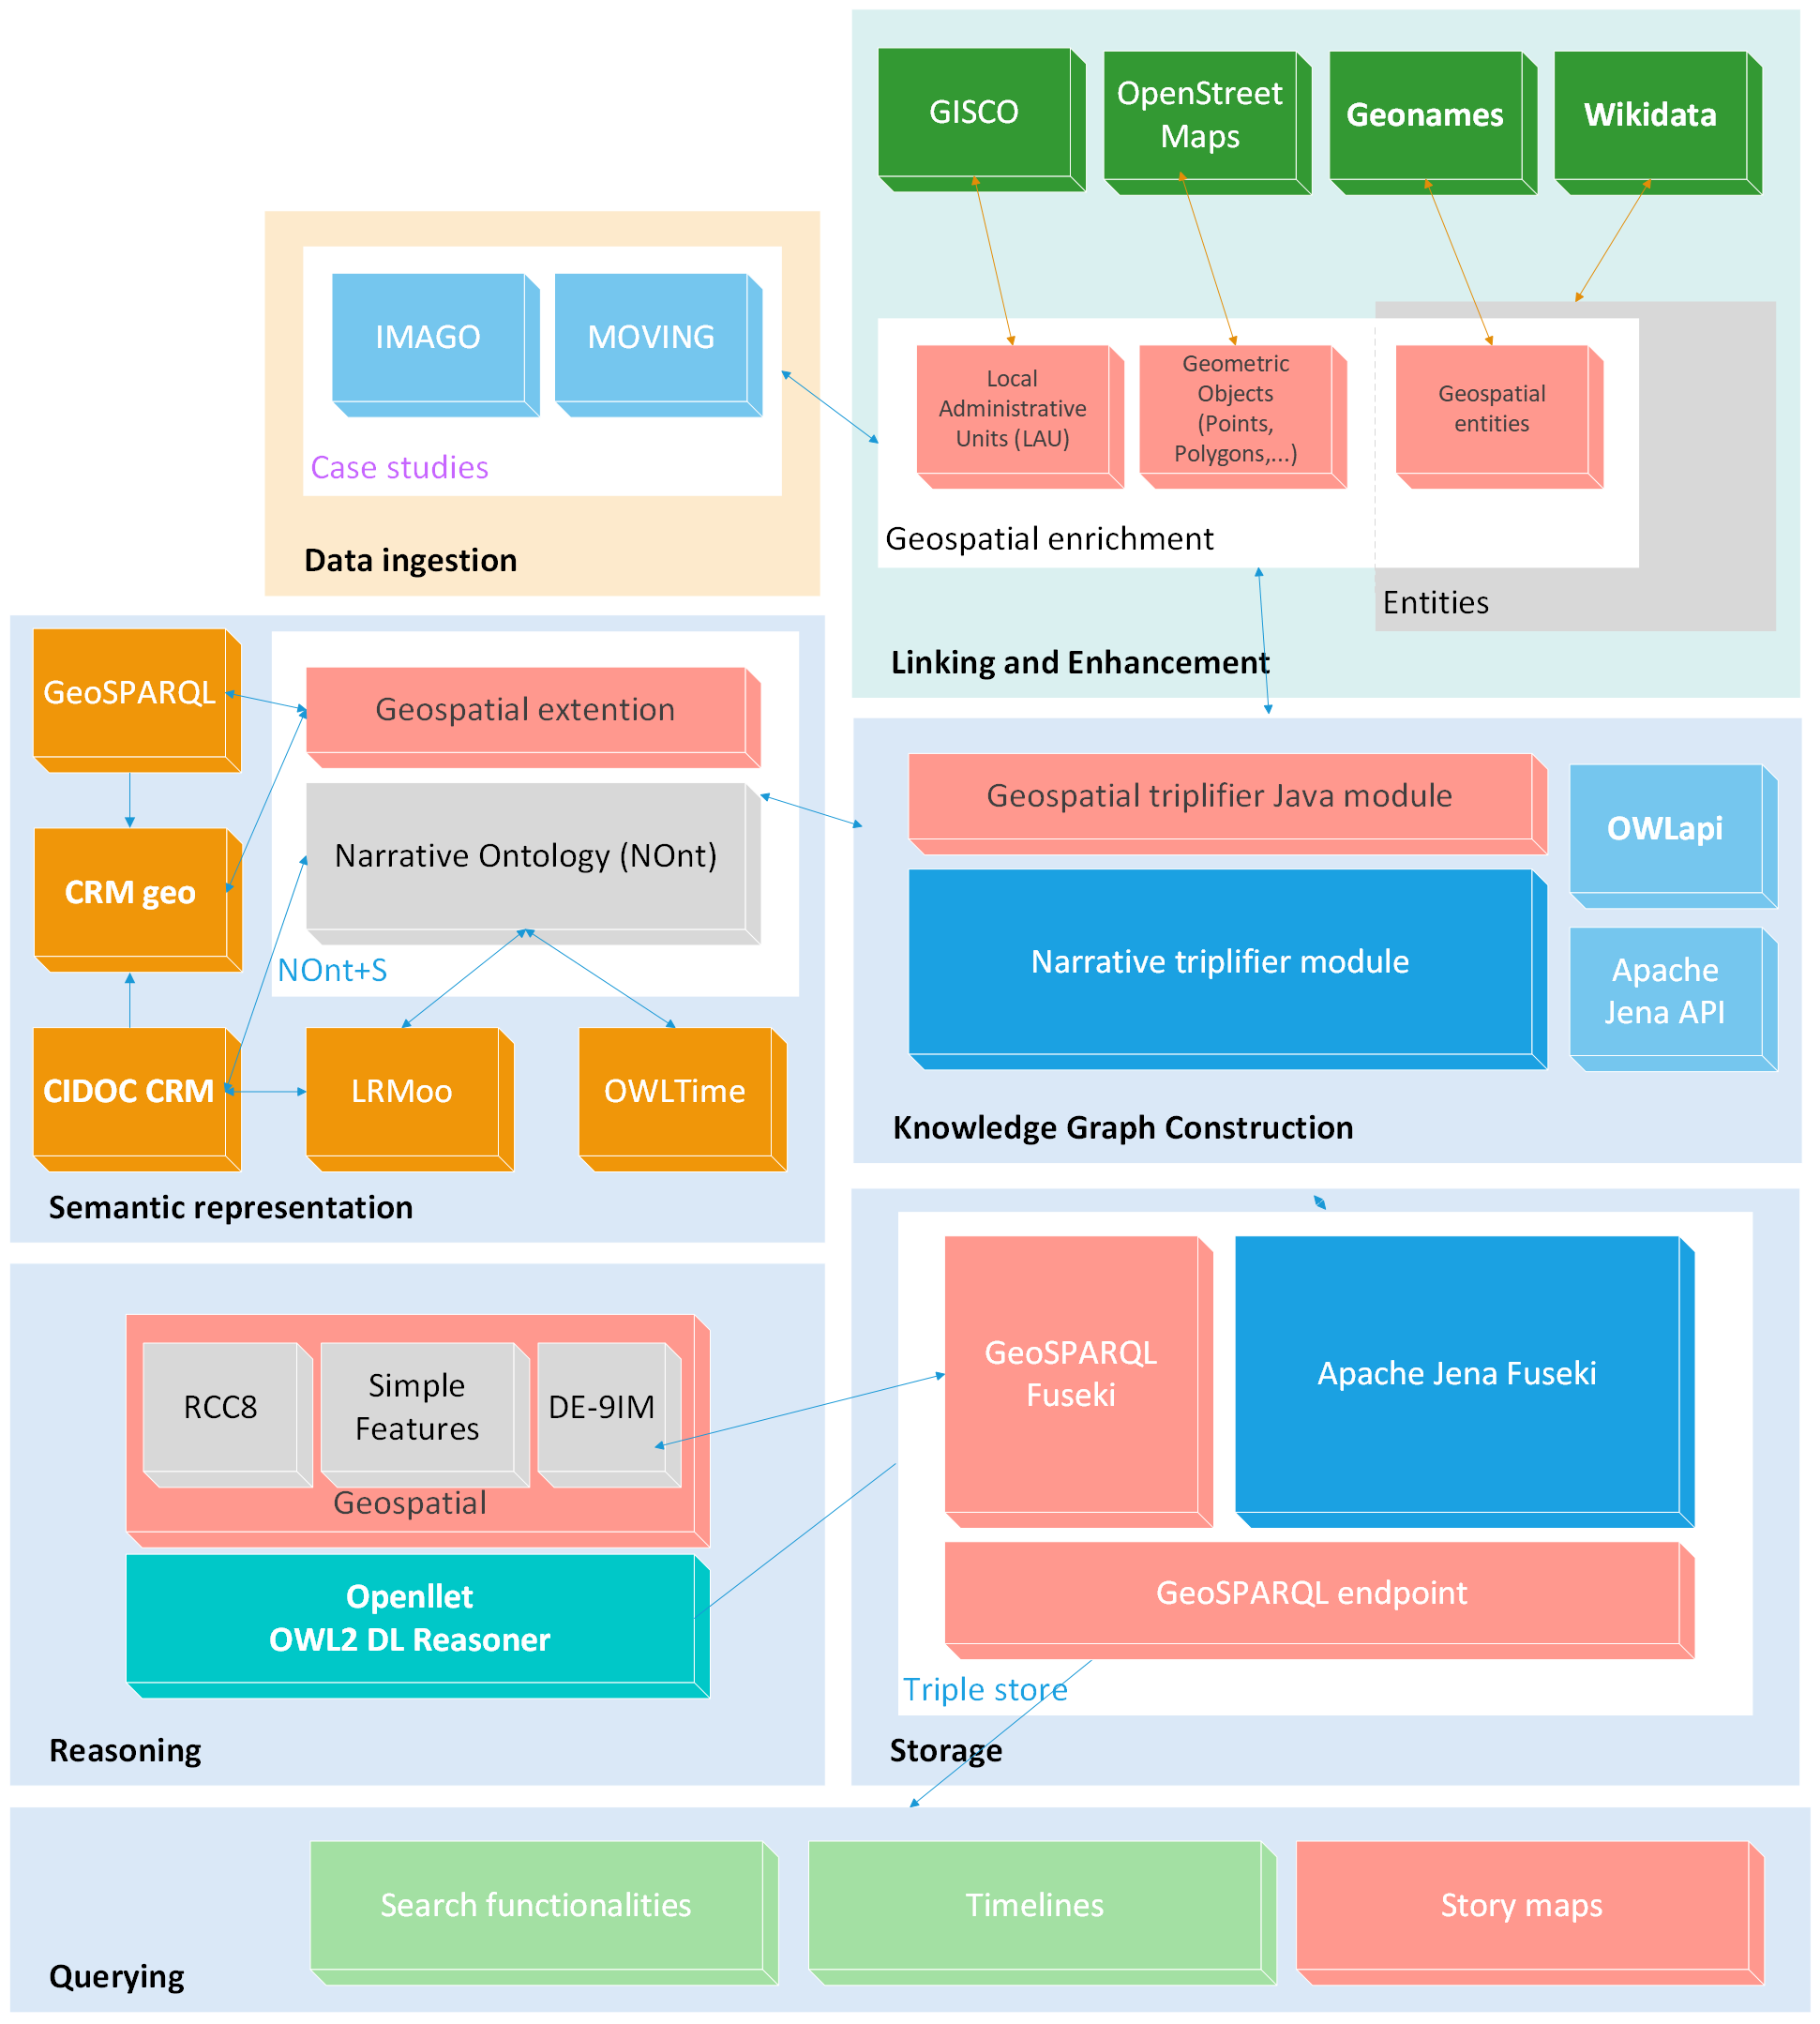
\includegraphics[scale=0.4]{img/SemanticFramework.png}}
    \caption{The image illustrates the semantic web framework of NOnt+S, highlighting its key components: data linking, semantic representation, knowledge graph construction, reasoning, triplestore storage, and advanced querying of geospatial data.}
    \label{fig:SemanticFramework}
\end{figure}

Each of these features is realized through modular components that interact to deliver a scalable and flexible system. The framework consists of six core modules that work in tandem to enable the effective use of geospatial data. These modules are designed to handle distinct tasks, from linking and enriching data to reasoning and querying it. Below, each module is described in detail.

\section{Linking and Enhancement}\label{VI-sec:linking}

The \textit{Linking and Enhancement} module is pivotal in constructing a unified and enriched knowledge graph by integrating data from diverse sources and augmenting it with additional semantic layers. This module ensures that the knowledge graph is both comprehensive and coherent, facilitating seamless integration of heterogeneous datasets into a single, enriched framework. The key tasks performed by this module include entity linking and data enrichment.

\subsection{Entity Linking}\label{VI-subsec:entitylinking}

Entity Linking (EL) is the process of connecting mentions of entities within datasets to their corresponding entities in a knowledge base. This task is essential for aligning semantically similar entities across different datasets, thereby enabling data integration and interoperability.

\subsubsection{Process of Entity Linking}

The entity linking process generally involves three main steps:

\begin{enumerate}
    \item \textbf{Entity Recognition}: Identifying and extracting entity mentions from the dataset. This involves natural language processing techniques to detect names, locations, organizations, and other entity types within unstructured or semi-structured data.
    \item \textbf{Candidate Generation}: For each extracted entity mention, generating a list of potential matching entities from the knowledge base. This step may use string matching, ontological mappings, or semantic similarity measures.
    \item \textbf{Entity Disambiguation}: Selecting the most appropriate entity from the candidate list by considering the context in which the entity mention appears. Techniques such as context vectors, machine learning classifiers, or probabilistic models are employed to determine the best match.
\end{enumerate}

\subsubsection{Linking to Wikidata}

An example of entity linking is connecting dataset entities to \textit{Wikidata} \cite{vrandecicWikidataFreeCollaborative2014}, an always up-to-date, community-driven, and multilingual knowledge base. Linking to Wikidata enriches the original data by incorporating a wealth of additional information, such as:

\begin{itemize}
    \item \textbf{Semantic Relationships}: Relationships between entities, enabling the inference of new knowledge through connected data.
    \item \textbf{Multilingual Labels}: Support for multiple languages, enhancing accessibility and usability across different linguistic communities.
    \item \textbf{Up-to-Date Information}: Continuous updates by a global community ensure that the data remains current.
\end{itemize}

By linking entities to a comprehensive knowledge base like Wikidata, the module enhances the semantic depth of the knowledge graph and promotes data interoperability.

The integration of information from diverse sources is essential in enhancing the quality and comprehensiveness of contemporary research and applications. Structured data repositories like \textit{Wikidata} \cite{vrandecicWikidataFreeCollaborative2014} and \textit{GeoNames} \cite{GeoNames} have become central to this ecosystem, offering extensive, collaboratively maintained datasets that support a wide range of use cases. While these repositories provide significant advantages, they also introduce challenges that necessitate careful consideration.

One of the most compelling strengths of \textit{Wikidata} is its role as a universal knowledge base. It offers structured data that is multilingual and compatible with linked data standards, enabling researchers to explore complex relationships between entities. Its collaborative nature ensures that information remains current and relevant, supported by contributions from a global community. Similarly, \textit{GeoNames} excels in providing rich geospatial data, including geographic coordinates, administrative hierarchies, and alternate place names. This repository is indispensable for applications such as geocoding, reverse geocoding, and geographic analysis, with seamless interoperability with Geographic Information Systems (GIS).

Despite their strengths, these repositories are not without limitations. The collaborative nature of \textit{Wikidata}, while a strength, also introduces potential inconsistencies and errors due to varying levels of expertise among contributors. The reliance on community-driven updates may lead to gaps in coverage or delays in incorporating critical information. \textit{GeoNames}, while rich in geospatial data, can sometimes lack granularity or fail to account for rapidly changing geopolitical landscapes. Furthermore, its reliance on standardized schemas may limit the ability to represent unique or culturally specific geographic distinctions.

The reliance on these repositories underscores both their value and the challenges they pose. On the one hand, they empower researchers and developers to access vast, structured datasets without the need to independently compile and validate such information. This reliance reduces resource demands and accelerates innovation. On the other hand, it raises questions about the reliability of the data and the risks of dependency on external platforms that may undergo policy changes or service disruptions. For projects requiring offline usability, reliance on live queries to \textit{Wikidata} or \textit{GeoNames} can pose significant challenges. Ensuring that essential datasets are locally replicated and periodically updated is critical to maintaining functionality in environments where internet connectivity is limited or unreliable.

\subsection{Enrichment}\label{VI-subsec:enrichment}

Enrichment involves augmenting the existing data with additional information to add value and context. In the context of this research, enrichment primarily focuses on adding geospatial information to entities, thereby introducing spatial dimensions to the datasets.


The enrichment process adds qualitative and quantitative spatial data to entities, which includes:

\begin{itemize}
    \item \textbf{Geographic Coordinates}: Adding latitude and longitude to pinpoint exact locations on the Earth's surface.
    \item \textbf{Polygons and Boundaries}: Defining the shape and extent of geographic entities, such as administrative regions, using polygon data.
    \item \textbf{Spatial Relationships}: Describing how entities are spatially related to one another, such as adjacency or containment relationships.
\end{itemize}

Enriching data with geospatial information brings numerous advantages that can significantly enhance the analysis and usability of datasets. One of the key benefits is the improvement in query capabilities. By incorporating spatial data, users can execute complex spatial queries, such as identifying entities within a specific radius or examining the spatial relationships between different entities. These queries allow for more dynamic and context-aware data analysis, which can be essential in applications like urban planning, environmental monitoring, or location-based services.

Another major advantage of geospatial data integration is its power in visualization and mapping. The ability to create detailed maps and spatial visualizations helps reveal patterns and insights that would otherwise remain hidden in non-spatial data. For example, geographic heat maps can highlight areas of high activity or risk, providing decision-makers with visual tools that translate complex data into actionable intelligence. Whether for business logistics, public health, or infrastructure development, geospatial visualizations make the interpretation of data more intuitive and impactful.

Additionally, geospatial enrichment allows for seamless integration with established geospatial standards, promoting compatibility with a wide array of data services. This is critical when working across various platforms or integrating datasets from multiple sources. Standards such as those from the Open Geospatial Consortium (OGC) ensure that enriched datasets can be shared and utilized in a broader context, fostering collaboration and enabling more extensive data interoperability across industries and governmental agencies.

Despite these advantages, the process of linking and enhancing data with geospatial information presents several challenges, each of which requires thoughtful solutions. One significant challenge is the ambiguity that arises when entities from different datasets need to be linked, especially when there are multiple possible matches in a knowledge base. To address this, context-aware disambiguation techniques are employed. Contextual similarity analysis, for instance, involves evaluating surrounding data or text to gather clues that help identify the correct entity. In addition, machine learning models can be trained on labeled datasets to predict the most probable entity matches. These models become increasingly sophisticated as they are exposed to more data, improving the accuracy of entity linking over time.

Another challenge stems from the fact that datasets sourced from various platforms often differ in format, schema, and overall quality. Standardization and normalization are critical processes to overcome these disparities. Aligning schemas involves using ontologies and data models to harmonize the data structures, ensuring that disparate datasets can be effectively merged or compared. Meanwhile, data cleaning techniques are employed to eliminate inconsistencies and errors, thereby enhancing the overall quality and reliability of the data. These processes ensure that the enriched dataset is not only comprehensive but also consistent and accurate, which is essential for any meaningful analysis.

Finally, processing large volumes of geospatial data requires substantial computational resources and efficient algorithms. To manage this, distributed computing frameworks such as Apache Hadoop or Spark can be utilized, enabling parallel processing across multiple nodes. This approach significantly reduces the time required for data processing, especially when handling big data. Additionally, the use of optimized algorithms with favorable time and space complexity ensures that operations are performed efficiently, minimizing computational overhead while maximizing performance. These solutions help address the scalability issues inherent in working with large datasets, ensuring that geospatial data enrichment can be applied even in resource-intensive environments.

By addressing these challenges with advanced techniques and solutions, the process of enriching data with geospatial information becomes more feasible, allowing organizations to unlock the full potential of their data for more informed decision-making.



\section{Semantic Representation}\label{VI-sec:semantic-representation}

At the core of the framework lies the \textit{Semantic Representation} module, which employs the NOnt+S ontology to structure and organize data. This module offers the formal representation of knowledge within narratives, ensuring that narrative concepts are accurately represented in the corresponding knowledge graph. A key feature of this module is its ability to integrate geospatial representations into the knowledge structure. As detailed in \ref{chap:nont+s}, the NOnt+S ontology provides an extensive and well-defined vocabulary for modeling geospatial entities, along with their associated attributes and relationships, thereby facilitating a comprehensive representation of both narrative and spatial elements within the semantic framework.

\section{Knowledge Graph Construction}\label{VI-sec:KG}

After the data has been semantically enriched and properly represented, the next crucial step involves the construction of the knowledge graph. This process is managed by the \textit{Knowledge Graph Construction} module, which is responsible for organizing the enriched data into a coherent graph-based structure. The purpose of this step is to translate the complex, interconnected information into a format that accurately represents geospatial entities and their relationships. The result is a formal structure using \acrshort{OWLLabel}2 DL (Web Ontology Language, Description Logic) \cite{OWLWebOntologyc}.

At the core of this process, the module utilizes two essential tools: the Apache Jena API\cite{ApacheJenaFramework} and the OWLapi\cite{OwlcsOwlapi2024}. Apache Jena is a widely-used framework that facilitates the creation and manipulation of RDF (Resource Description Framework) graphs, while OWLapi is specifically designed to handle \acrshort{OWLLabel} ontologies. Together, these technologies form the backbone of the knowledge graph construction process, enabling the seamless conversion of the enriched data into a robust, ontology-based structure.

One of the module's key components, the \textit{triplifier} software, plays a significant role in this transformation. The triplifier software converts the enriched data into RDF triples, the building blocks of the knowledge graph. These triples represent subject-predicate-object relationships, providing a flexible and scalable means of capturing complex data. 

Particularly noteworthy is the role of the \textit{geospatial triplifier} software within the module. This specialized component is designed to manage geospatial data by facilitating the conversion between various spatial data formats, such as \acrfull{WKTLabel}\cite{WellknownTextRepresentationa} and \acrfull{GMLLabel}\cite{GeographyMarkupLanguagea}. WKT and GML are common standards for representing spatial information, and their compatibility with the knowledge graph format is essential for ensuring that the spatial relationships between entities are maintained and accurately reflected in the graph. Through this process, the geospatial triplifier software enables the seamless integration of location-based data into the overall knowledge graph, allowing for sophisticated queries and reasoning over geospatial entities and their interconnections.

\section{Reasoning}\label{VI-sec:reasoning}

The \textit{Reasoning} module is a critical component of the framework, enabling semantic reasoning, which is the process of deriving new insights from existing data. This ability to infer new facts is based on predefined inference rules or ontologies, allowing for the enrichment of the knowledge graph. By introducing new knowledge and adding context, the module enhances the dataset’s depth and usability. The Reasoning module goes beyond mere data retrieval; it transforms a static repository into an intelligent system capable of generating additional information and insights from the given data. Furthermore, it integrates geospatial reasoning, extending its utility to spatial data and relationships.

The Reasoning module provides two key capabilities that empower the framework to extend the meaning and utility of the data: Geospatial Reasoning and Semantic Reasoning.

\subsection{Geospatial Reasoning}\label{VI-subsec:geospatialReasoning}

Geospatial reasoning is a critical component of the framework, as it enables the system to derive meaningful inferences about spatial relationships and configurations from annotated geographical data. This form of reasoning extends beyond simple location retrieval; it encompasses the ability to interpret spatial properties and to draw both quantitative and qualitative conclusions about the relative positions, distances, and spatial hierarchies among entities. By harnessing geospatial reasoning, the system can address complex queries, such as identifying proximity between historical sites, detecting overlaps in territorial boundaries, or establishing containment relationships between regions.

The process of geospatial reasoning integrates seamlessly with the GeoSPARQL standard, which provides a robust model for representing and querying geospatial information within OWL graphs. GeoSPARQL’s capabilities facilitate the interpretation of both explicit geospatial data, such as coordinates or polygon geometries, and implicit spatial relationships that can be inferred through reasoning mechanisms. For example, when analyzing medieval or Renaissance geographical texts, the system can infer that a particular site lies within a specified historical region based on its coordinates or can recognize spatial patterns among multiple places that share a common historical significance.

\subsection{Semantic Reasoning}\label{VI-subsec:semanticReasoning}

Reasoning within OWL 2 DL is a cornerstone of its utility in the Semantic Web, primarily because of its formal grounding in Description Logics (DLs) that ensures decidability and expressiveness. OWL 2 DL is designed to balance the trade-off between computational complexity and the need for a rich modeling language. It enables reasoning over ontologies by leveraging a complete model-theoretic semantics, allowing inferential tasks such as subsumption checking, instance classification, and consistency verification. This is achieved through the incorporation of advanced logical constructs derived from the SROIQ description logic, which supports features like role hierarchies, qualified cardinality restrictions, and rich property characteristics, including inverses, chains, and transitivity. The adoption of DL semantics guarantees that every valid inference can be systematically derived, ensuring predictability and reliability. Moreover, OWL 2 DL imposes syntactic restrictions that segregate entities like classes, properties, and individuals, thereby avoiding the ambiguity of interpretation inherent in RDF-based semantics. These restrictions are crucial for preserving the decidability of reasoning tasks. By combining expressive power with algorithmic feasibility, OWL 2 DL provides a robust framework for developing interoperable and logically sound ontologies, making it an indispensable tool for the realization of the Semantic Web's vision of a machine-understandable web of knowledge.

Reasoners for OWL 2 DL ontologies serve as critical components in semantic web technologies, facilitating various forms of reasoning essential for ontology-based applications. This section provides a short analysis of these reasoners, but a deeper analysis on what reasoners are still usable can be found in \cite{abichtOWLReasonersStill2023}. 

\subsubsection{FaCT++}
FaCT++\cite{tsarkovFaCTDescriptionLogic2006} is a highly optimized OWL 2 DL reasoner that succeeds the original FaCT (Fast Classification of Terminologies). It implements a tableaux decision procedure for SHOIQ Description Logic and extends support to data types such as strings and integers. The latest version (1.6.5) is available on a Bitbucket repository, with the last commit made in December 2017. While FaCT++ is integrated into the standard Protégé 5.6.1 distribution, standalone downloads are also available. Despite occasional plugin installation issues on Windows, documented workarounds ensure usability, and its consistent use in research underscores its reliability.

\subsubsection{HermiT}
HermiT \cite{glimmHermiTOWL22014} is a Java-based OWL 2 reasoner that employs hypertableau calculus to provide entailment checking and other reasoning services such as class and property classification, as well as SPARQL query answering. While its development has ceased (with the latest version, 1.3.8, available on a GitHub repository), it remains accessible as a plugin in Protégé 5.6.1. Although official binaries are scarce, unofficial options exist, ensuring its usability. HermiT's historical significance and functionality make it a mainstay for reasoning tasks within OWL 2 ontologies.

\subsubsection{JFact}
JFact \cite{JFactDLReasoner} is a Java port of FaCT++, designed for compatibility with OWL API 3.x and 4.x. Although no dedicated publications describe JFact, it has been referenced in academic literature and provides downloadable resources from GitHub and SourceForge. While its compatibility with Protégé 5.6.1 remains partially uncertain, JFact functions effectively within Java projects. This portability and alignment with the OWL API make it a suitable choice for developers seeking to leverage FaCT++'s capabilities in Java environments.

\subsubsection{Openllet}
Openllet \cite{galigatorGaligatorOpenllet2024}, a fork of Pellet, extends and optimizes reasoning functionality for OWL 2. It supports tasks such as consistency checking, classification hierarchy computation, inference explanation, and SPARQL query answering. Openllet's latest version (2.6.5) is actively maintained, with the most recent update in May 2023. Distributed as an open-source project, it offers pre-generated JAR files and example usage documentation. While a Protégé plugin is mentioned, it appears to lack widespread availability. Openllet’s focus on optimization and modern compatibility makes it ideal for performance-intensive reasoning tasks.

\subsubsection{Pellet}
Pellet \cite{sirinPelletPracticalOWLDL2007} has the distinction of being one of the first sound and complete OWL 2 DL reasoners. Written in Java, it supports a comprehensive suite of reasoning tasks, including debugging ontologies and reasoning with user-defined data types. While its original website is no longer accessible, several GitHub repositories provide source code. However, these repositories are no longer actively maintained. Despite this, Pellet remains usable via its integration into Protégé 5.6.1, where it serves as a reliable reasoning tool for ontology-based applications. Its legacy and functionality ensure its relevance, especially for applications requiring debugging and data type reasoning.

\subsubsection{Chainsaw}
Chainsaw \cite{tsarkovChainsawMetareasonerLarge} is a meta-reasoner designed to handle large ontologies by generating modules and delegating reasoning tasks to specialized third-party reasoners, such as ELK. Its modular decomposition approach is particularly effective for scalability and performance optimization. The Chainsaw source code is available on a Bitbucket repository, with the latest commit recorded in 2022. Downloads are hosted on SourceForge, ensuring accessibility for researchers and developers seeking a scalable solution to ontology reasoning.

\subsection{The Integration of Openllet in the Framework}

Pellet, and its open-source counterpart Openllet, have emerged as prominent reasoning engines for OWL 2 DL ontologies, providing robust capabilities that make them indispensable for numerous semantic web applications. These reasoners support essential inference tasks, including subsumption, consistency checking, and instance realization, all of which are foundational for enabling intelligent query answering and ensuring semantic coherence in ontology-driven systems.

While most OWL 2 DL reasoners are primarily designed to operate within the Protégé environment \cite{musenProtegeProject2015}, their adaptability to other platforms can vary significantly. This limitation often constrains the broader applicability of such tools in diverse frameworks that rely on alternative storage and query mechanisms. Our framework, detailed further in Section \ref{VI-sec:storage}, leverages the Fuseki API to provide efficient RDF data storage and SPARQL querying capabilities. Openllet distinguishes itself as the only reasoning engine fully compatible with Fuseki, ensuring seamless integration for performing reasoning tasks directly within this environment. 

Moreover, Openllet extends its utility by supporting GeoSPARQL within Fuseki, a critical feature for applications that incorporate geospatial data. This compliance facilitates advanced geospatial reasoning, enabling operations such as spatial relationships and topology-based queries to be executed with the same semantic rigor as standard OWL reasoning. The ability to bridge the reasoning needs of OWL 2 DL with geospatial data requirements highlights Openllet’s unique position within the ecosystem of semantic web technologies, reinforcing its suitability for integration into our framework.

This synergy between Openllet and Fuseki not only broadens the functional scope of the reasoning process but also enhances the scalability and flexibility of the framework, making it well-suited for a wide range of semantic web and geospatial applications.


\section{Storage}\label{VI-sec:storage}

In the domain of knowledge representation and the Semantic Web, triplestores play a fundamental role in storing and querying structured data. 
In modern knowledge representation systems, managing enriched and semantically structured data requires an efficient, scalable, and reliable storage solution. This chapter describes the storage module of the framework, which leverages a triplestore to handle \acrshort{OWLLabel} triples that form the backbone of the knowledge graph. A triplestore is a database specifically designed for storing and managing \acrshort{RDFLabel}/\acrshort{OWLLabel} triples, making it particularly well-suited for knowledge graphs that require efficient querying, scalability, and the ability to manage complex, interconnected datasets.

A triplestore serves as the fundamental storage component of the framework, managing \acrshort{OWLLabel} triples, where each triple consists of a subject, predicate, and object. This structure allows for the flexible representation of relationships and properties in a semantic format, enabling sophisticated knowledge representation. In the context of this framework, the triplestore ensures that the knowledge graph remains accessible and performant, even as it scales to accommodate large and complex datasets, such as geospatial data. The Storage module is designed with two critical capabilities: efficient data retrieval and scalability. These features ensure the triplestore can handle the demands of storing and querying semantically rich, interconnected data. Triplestores are optimized for querying large volumes of \acrshort{RDFLabel} triples, making them ideal for use cases that involve extensive, highly interconnected data, such as geospatial knowledge graphs. The framework utilizes \acrshort{SPARQLLabel}\cite{ericprudhommeauxSPARQLQueryLanguage2008}, a powerful query language specifically designed for \acrshort{RDFLabel} data, to retrieve information from the triplestore. The inherent efficiency of triplestores in executing complex queries enables fast data retrieval, even in scenarios where relationships span numerous triples. As the amount of data ingested into the system grows, the triplestore must scale accordingly. The framework's triplestore is designed to handle increasing volumes of \acrshort{OWLLabel} triples without compromising performance. This scalability is particularly important for knowledge graphs in domains such as geospatial analysis, where large datasets are common, and the ability to maintain performance with growing data volumes is critical.

\subsection{Implementation: Fuseki and GeoSPARQL Support}\label{VI-subsec:fuseki}

Fuseki is the triplestore component of the Apache Jena framework, an open-source and widely adopted Java-based platform for building Semantic Web applications \cite{ApacheJenaFramework}. As part of Apache Jena, Fuseki provides robust capabilities for storing, managing, and querying \acrshort{RDFLabel} datasets, specifically through its support for the \acrshort{SPARQLLabel} query language \cite{ApacheJenaFuseki}. It is particularly well-suited for Semantic Web use cases, where \acrshort{RDFLabel} serves as the foundational data model and \acrshort{SPARQLLabel} as the query language. Fuseki offers key features that facilitate efficient data management and retrieval for Semantic Web projects:

\begin{itemize}
    \item \textbf{\acrshort{SPARQLLabel} 1.1 Compliance}: Fuseki fully implements the \acrshort{SPARQLLabel} 1.1 standard, enabling comprehensive support for various query types such as SELECT, CONSTRUCT, ASK, and UPDATE, thereby allowing sophisticated interaction with \acrshort{RDFLabel} data.
    \item \textbf{HTTP Protocol Integration}: It provides an HTTP interface, enabling \acrshort{SPARQLLabel} queries to be executed and results retrieved over the web, which is particularly useful for web-based Semantic Web applications.
    \item \textbf{Flexible Data Storage}: Fuseki supports multiple storage options, including in-memory and persistent stores, giving developers the flexibility to choose the appropriate storage backend based on application requirements.
    \item \textbf{Modularity and Extensibility}: Highly modular by design, Fuseki allows for easy extension with custom functionalities, enabling developers to incorporate additional data processing standards such as GeoSPARQL \cite{GeoSPARQLFuseki}.
\end{itemize}

As outlined in chapter \ref{chap:theoretical_framework}, GeoSPARQL is an OGC standard designed to extend SPARQL with the capability to represent and query geospatial data. It introduces geospatial vocabularies, filters, and topological functions, allowing \acrshort{RDFLabel} datasets to manage spatial information \cite{matthewperryOGCGeoSPARQLGeographic2012}. The GeoSPARQL Fuseki extension integrates this standard into the Fuseki triplestore, enabling the execution of geospatial queries through the standard Fuseki HTTP server or as an embedded component \cite{GeoSPARQLFuseki}. This extension ensures full compliance with the GeoSPARQL standard, allowing users to perform spatial queries on \acrshort{OWLLabel} datasets using \acrshort{SPARQLLabel} enriched with geospatial functions. 

GeoSPARQL Fuseki’s HTTP interface supports all relevant GeoSPARQL predicates and functions, simplifying its integration with existing web services and applications. Furthermore, its modularity allows it to be embedded within Fuseki’s core, enabling developers to add geospatial querying capabilities to their \acrshort{RDFLabel} datasets without the need to run a separate service. This adaptability underscores Fuseki's strength in supporting diverse and evolving needs within Semantic Web and geospatial data applications.

\subsection{GeoSPARQL Compliance Testing}\label{VI-subsec:compliance-geosparql}

To ensure that the triplestore implementation adheres to the required standards, we conducted a GeoSPARQL compliance test. Compliance with GeoSPARQL guarantees that a triplestore can effectively store, manage, and query geospatial data in line with the requirements established by GeoSPARQL \acrshort{OGCLabel} standard\cite{GeoSPARQLGeographicQuerya}. Verifying compliance involves benchmarking the system against a set of criteria defined by the GeoSPARQL specification. Jovanovik et al. \cite{jovanovikGeoSPARQLComplianceBenchmark2021a} proposed a benchmark designed to evaluate the compliance of various triplestores with the GeoSPARQL standard. When our implementation was tested using this framework, the results showed a compliance level comparable to those reported in prior studies, confirming that our triplestore meets many of the core GeoSPARQL requirements. However, the results also revealed that certain aspects of the GeoSPARQL specification are not fully supported by the triplestore.

\begin{table}[ht]
\centering \caption{Triplestore Feature Comparison}
\label{tab:triplestore-comparison}
\vskip 0.2cm
\scalebox{0.90}{
\begin{tabular}{|l|c|c|c|c|c|c|}
\hline
\textbf{Triplestore}      & \textbf{CORE} & \textbf{TOP} & \textbf{GEOEXT}               & \textbf{GTOP}                 & \textbf{RDFSE} & \textbf{QRW}  \\ \hline
GeoSPARQL Fuseki          & Full          & Full         & Full/E                        & Full                          & Full           & Full/E        \\ \hline
GraphDB          & Full          & Full         & Partial [WKT]                 & Partial [WKT]                 & Full           & None          \\ \hline
Strabon          & Full          & Full         & Partial [WKT]                 & Partial [WKT]                 & Full           & None          \\ \hline
Virtuoso         & Full          & Full         & Partial [WKT]                 & Partial [WKT]                 & Full           & None          \\ \hline
TriplyDB                  & Full          & Full         & Partial [WKT]                 & Partial [WKT]                 & Full           & None          \\ \hline
RDF4J   c          & Full          & Full         & Partial [WKT CRS84]           & Partial [WKT CRS84]           & Full           & None          \\ \hline

\end{tabular}
}
\end{table}

In addition, we applied\footnote{The code for replicating the evaluation is available on GitHub at \url{https://github.com/prate91/Geosparql2benchmark}} the benchmark to Strabon, a system not previously evaluated by Jovanovik et al., which supports both GeoSPARQL and stSPARQL\cite{koubarakisModelingQueryingMetadata2010a}. To better understand the variations in compliance across different systems, we analyzed the benchmark results with respect to the six extensions defined in the GeoSPARQL specification. Table \ref{tab:triplestore-comparison} summarizes the results for major triplestores that support at least partial implementations of the Geometry Extension (GEOEXT) and Geometry Topology (GTOP). The core components and extensions of GeoSPARQL are briefly described as follows. The Core component (CORE) defines the foundational spatial vocabulary elements, while the Topology vocabulary extension (TOP) specifies the vocabulary for topological relations. The Geometry Extension (GEOEXT) provides vocabulary for geometry and non-topological query functions, and the Geometry Topology extension (GTOP) defines topological query functions for geometry objects. The \acrshort{RDFSLabel} Entailment Extension (RDFSE) introduces mechanisms to match inferred RDF triples based on \acrshort{RDFLabel} and \acrshort{RDFSLabel} semantics, enabling reasoning through \acrshort{RDFSLabel}. Finally, the Query Rewrite extension (QRW) specifies rules for transforming queries to compute spatial relations between objects based on their geometries.

Among the triplestores tested, GeoSPARQL Fuseki demonstrated the highest level of compliance, consistently outperforming other systems in overall GeoSPARQL support. It was the only triplestore that fully supported both \acrshort{GMLLabel} and \acrshort{WKTLabel} formats, as well as the only one that implemented all GeoSPARQL extensions. However, despite these strengths, GeoSPARQL Fuseki exhibited certain limitations during the benchmark tests. Specifically, it returned incorrect results for certain functions within the Query Rewrite (QRW) and Geometry (GEOEXT) extensions. These issues indicate the need for further optimization to fully support advanced GeoSPARQL functionalities, particularly in the areas of geometry handling and query rewriting.

A significant problem identified by the benchmark was GeoSPARQL Fuseki’s inability to handle empty WKT and GML literals—an issue observed across all triplestores tested. Proper handling of empty literals is essential for ensuring robust GeoSPARQL support, as it directly impacts the accuracy and reliability of query results, particularly when working with complex geospatial datasets. Addressing this limitation is critical for enhancing the overall reliability and functionality of GeoSPARQL implementations.

\subsection{Performance Benchmarking with GeoSPARQL Fuseki}\label{VI-subsec:performance-geosparql}

In addition to compliance testing, the performance of the framework with GeoSPARQL Fuseki was evaluated using the benchmarking tool \textit{Geographica 2}\cite{ioannidisEvaluatingGeospatialRDF2021}. This benchmark is designed to assess the performance of triplestores in processing geospatial queries, with a particular focus on query execution time and scalability when handling large geospatial datasets. While many triplestores such as Strabon, uSeek, Parliament, System X, GraphDB, and RDF4J have been tested with this benchmark, GeoSPARQL Fuseki has not yet been evaluated within this framework.

We implemented the test of GeoSPARQL Fuseki in two distinct configurations to assess its performance in two differents use cases. The first one is in localhost on windows, trying to assess the performance without the connection to a server (configuration 1). The second configuration is on a server platform served through tomcat9, accessible through an endpoint. The two configurations are shown in Table \ref{tab:triplestore-performance-configuration}:

\begin{table}[ht]
\centering \caption{System Configurations for GeoSPARQL Fuseki Performance Testing}
\label{tab:triplestore-performance-configuration}
\vskip 0.2cm
\scalebox{0.90}{
\begin{tabular}{|l|c|c|}
\hline
\textbf{Component}          & \textbf{Configuration 1}                                    & \textbf{Configuration 2}                                    \\ \hline
\textbf{Platform}           & Windows 10.0.22635 (AMD64)                                  & Linux (Ubuntu 5.15.0-117-generic)                           \\ \hline
\textbf{Processor Model}    & 11th Gen Intel\textsuperscript{\tiny\textregistered} Core\textsuperscript{\texttrademark} i7-1165G7                        & Intel\textsuperscript{\tiny\textregistered} Xeon\textsuperscript{\tiny\textregistered} CPU E5-4610 v2                             \\ \hline
\textbf{Base Frequency}     & 2.80 GHz                                                    & 2.30 GHz                                                    \\ \hline
\textbf{Architecture}       & x86-64 (AMD64)                                              & x86-64                                                      \\ \hline
\textbf{Microarchitecture}  & Tiger Lake                                                  & Ivy Bridge                                                  \\ \hline
\textbf{Physical Cores}     & 4                                                           & 2                                                           \\ \hline
\textbf{Total Cores}        & 8                                                           & 2                                                           \\ \hline
\textbf{RAM}                & 16 GB                                                       & 16 GB                                                       \\ \hline
\end{tabular}
}
\end{table}

Before presenting the results of this benchmark on the two configurations, we briefly present the relevant concepts of the Geographica2 benchmark. For a comprehensive explanation of the benchmark and its full evaluation, please refer to Ioannidis et al. \cite{ioannidisEvaluatingGeospatialRDF2021}. The benchmark tests real-world, synthetic, and scalability workloads, each focusing on different aspects of \acrshort{RDFLabel} store performance.

To benchmark \acrshort{RDFLabel} stores accurately, Geographica 2 uses a variety of datasets, including real-world data from \acrfull{LODLabel} and specialized datasets with complex geometries. These datasets help simulate real-world geospatial tasks and provide the basis for the workloads. The real datasets employed by the benchmark are divided into three groups: \acrshort{LODLabel} datasets, datasets with complex geometries and specialized datasets. In the first group, there is (i) DBpedia\cite{DBpedia2024}, a crowd-sourced knowledge base derived from Wikipedia that contains geospatial information in the form of point geometries (e.g., cities, buildings); (ii) GeoNames\cite{GeoNames}, a global geographical database with over 11 million unique features that provide point geometries representing cities, lakes, and landmarks, with coordinates in the WGS84 \acrshort{CRSLabel}, and \acrfull{LGDLabel}\cite{LinkedGeoData}, based on \acrfull{OSMLabel}\cite{OpenStreetMap} that includes features such as motorways, rivers, and geographic entities. Then, in the second group, there is (i) \acrfull{GAGLabel}\cite{GreekAdministrativeGeography}, a dataset containing polygon geometries representing municipalities in Greece, crucial for spatial join operations; (ii) \acrfull{CLCLabel}\cite{CORINELandCover}, a dataset from the European Environmental Agency with complex polygon geometries representing land cover across Europe; and (iii) Wildfire Hotspot Dataset\cite{sifakisWildfireDetectionTracking2011}, developed by the National Observatory of Athens that consists of polygons representing wildfire areas, derived from \acrfull{EOLabel} data. Finally, the third group is compose only by Census Dataset, sourced from the U.S. Census Bureau, includes the street network data of New York City. Streets are represented as linestrings, with detailed address ranges, enabling geocoding operations.

The real datasets are employed in the real-world workload that simulates common geospatial tasks in order to evaluate how efficiently stores handle geospatial queries involving \acrshort{LODLabel}, spatial joins, and polygon and point operations. The real-world workload is divided into micro benchmark and macro benchmark. The micro benchmark tests the efficiency of basic spatial functions in geospatial triplestores using simple GeoSPARQL queries. The comprehensive set of queries designed for evaluating the performance of geospatial systems, as discussed in \cite{ioannidisEvaluatingGeospatialRDF2021}, comprises 29 distinct queries. These queries are systematically categorized into four primary groups. However, for our performance assessment using Fuseki GeoSPARQL, we limited the evaluation to three of these groups, excluding the fourth, which focuses on Aggregate Functions\footnote{The queries for this group are available at \url{https://geographica2.di.uoa.gr/queries/micro_aggregations.lst}}. This group (Q28 and Q29) exclusively utilizes the stSPARQL operator and is thus not pertinent to our comparative analysis. Specifically, the first group, denoted as \acrfull{NTCFLabel}\footnote{The queries for this group can be accessed at \url{https://geographica2.di.uoa.gr/queries/micro_nontopological.lst}}, encompasses queries Q1 to Q6 and addresses non-topological conditions. The second group, labeled as \acrfull{SSLabel}\footnote{The queries for this group are available at \url{https://geographica2.di.uoa.gr/queries/micro_selections.lst}}, spans from Q7 to Q17, focusing on selection-based geospatial queries. Finally, the third group, \acrfull{SJLabel}\footnote{The queries for this group can be consulted at \url{https://geographica2.di.uoa.gr/queries/micro_joins.lst}}, includes queries Q18 to Q27, which are structured around join operations within geospatial datasets.
The macro benchmark evaluates geospatial triplestores in complex real-world applications, such as geocoding, reverse geocoding, map search and browsing, and earth observation scenarios.

There is also a synthetic workload that tests system performance using artificially generated datasets and queries. This workload includes two key metrics: data scalability, which tests the system's response as the dataset size increases, and query selectivity, which evaluates performance based on varying levels of query selectivity. In this workload, the queries are built based on the query template shown in \ref{lst:template-synthetic} to produce SPARQL queries corresponding to spatial selections that ask for land ownerships which intersect a given rectangle and points of interest that are within a given rectangle. The given rectangle is generated in such a way that the spatial predicate of the query holds for 0.01\%, 10\%, 25\%, 50\%, or 75\% of all the features of the respective dataset. In addition, the query template was instantiated using the extreme values 1 and 512 for the parameter THEMA, selecting either all or approximately 0.02\% of the total features of a dataset.

\begin{lstlisting}[caption=Template to build queries for synthetic workload from \cite{ioannidisEvaluatingGeospatialRDF2021}, label={lst:template-synthetic}]
 SELECT ?s
    WHERE{ 
    ?s ns:hasGeometry/ns:asWKT ?g.
    ?s c:hasTag/ns:hasKey "THEMA".
    FILTER(FUNCTION(?g, "GEOM"))}
\end{lstlisting}

Eventually, there is the Scalability Workload that assesses how the system handles increasingly large datasets. The metrics include storage efficiency, evaluating how efficiently large datasets are stored, bulk loading time, measuring the time to load large datasets and query response Time, and analyzing how query performance scales as data volume increases.

\subsection{Geographica2 Results for GeoSPARQL Fuseki}\label{VI-subsec:geographica2-results}

The evaluation results\footnote{The code for replicating the evaluation is available on GitHub at \url{https://github.com/prate91/Geosparql2benchmark} and \url{https://github.com/prate91/geographica2}} indicate that GeoSPARQL Fuseki demonstrates strong performance across various types of geospatial queries, affirming its capability to handle increased geospatial data efficiently. This efficiency positions it as a suitable choice for real-time analysis within the Semantic Web framework. A detailed examination of the data reveals several patterns in performance based on query type and specific query configurations.

In \acrshort{NTCFLabel}, GeoSPARQL Fuseki outperformed other triplestores in many cases, particularly from Q2 to Q6. This advantage highlights its capability to manage non-topological query processing with notable efficiency, a critical aspect for systems requiring rapid responses to spatial data without complex relational dependencies. The configuration variations of Fuseki also show consistent improvement, with configuration 2 slightly surpassing configuration 1 in response times across these queries.


 \begin{table}[h!tb]
   \centering \caption{Performance (seconds) of Triple Stores.
The symbols represent performance percentiles: \ding{115} indicates values between the 33rd and 67th percentiles, \ding{108} denotes values below the 33rd percentile, and \ding{110} represents values above the 67th percentile. Performance data for triple stores other than Fuseki is sourced from the Geographica2 benchmark.}
\label{table:cold_caches}
   \vskip 0.2cm
   %%
   \scalebox{0.90}{
	    %% The {|c|c|c|c|c|} define the number of columns.
	    %% c means centered
	    %% | defines a vertical line between two columns 
	    \begin{tabular}{|c|c|r|r|r|r|r|r|}
        \hline
	     Type & Query & Strabon & GraphDB & RDF4J & RDF4J (L) & Fuseki (c1) & Fuseki (c2) \\ \hline
NTCF & Q1 & \ding{115} 42.33 & \ding{108} 29.68 & \ding{115} 37.24 & \ding{115} 37.34 & \ding{110} 50.78 & \ding{110} 52.44 \\
              & Q2 & \ding{110} 22.48 & \ding{108} 14.55 & \ding{115} 18.41 & \ding{115} 18.75 & \ding{108} 12.24 & \ding{110} 25.31 \\
              & Q3 & \ding{110} 29.48 & \ding{108} 19.42 & \ding{115} 24.57 & \ding{115} 24.56 & \ding{108} 18.26 & \ding{110} 31.04 \\
              & Q4 & \ding{110} 7.65 & \ding{108} 3.20 & \ding{108} 3.32 & \ding{108} 3.48 & \ding{108} 2.72 & \ding{108} 4.26 \\
              & Q5 & \ding{110} 14.68 & \ding{115} 7.45 & \ding{108} 4.52 & \ding{108} 4.64 & \ding{108} 3.00 & \ding{108} 4.46 \\
              & Q6 & \ding{110} 23.82 & \ding{115} 13.53 & \ding{110} - & \ding{110} - & \ding{108} 0.25 & \ding{108} 0.17 \\ \hline
SS & Q7 & \ding{108} 0.36 & \ding{110} 5.33 & \ding{115} 3.64 & \ding{110} 3.97 & \ding{110} 5.71 & \ding{108} 0.77 \\
              & Q8 & \ding{108} 0.42 & \ding{110} 2.04 & \ding{110} 1.76 & \ding{110} 1.78 & \ding{110} 2.36 & \ding{115} 1.67 \\
              & Q9 & \ding{108} 0.83 & \ding{110} 28.28 & \ding{110} 40.46 & \ding{110} 40.60 & \ding{110} 38.42 & \ding{108} 3.75 \\
              & Q10 & \ding{108} 0.73 & \ding{110} 22.24 & \ding{110} 25.40 & \ding{110} 25.24 & \ding{110} 19.74 & \ding{110} 23.61 \\
              & Q11 & \ding{108} 2.66 & \ding{110} 114.29 & \ding{110} 164.48 & \ding{110} 164.84 & \ding{110} 154.94 & \ding{108} 35.76 \\
              & Q12 & \ding{115} 0.79 & \ding{110} 1.02 & \ding{108} 0.65 & \ding{108} 0.67 & \ding{115} 0.80 & \ding{108} 0.63 \\
              & Q13 & \ding{108} 0.82 & \ding{110} 49.67 & \ding{110} 72.89 & \ding{110} 72.20 & \ding{110} 70.89 & \ding{108} 6.74 \\
              & Q14 & \ding{108} 0.50 & \ding{108} 4.13 & \ding{108} 1.85 & \ding{108} 1.90 & \ding{110} 63.84 & \ding{108} 7.08 \\
              & Q15 & \ding{108} 0.50 & \ding{110} 0.93 & \ding{108} 0.44 & \ding{108} 0.48 & \ding{115} 0.67 & \ding{108} 0.58 \\
              & Q16 & \ding{108} 2.79 & \ding{115} 50.61 & \ding{110} 72.86 & \ding{110} 72.34 & \ding{110} 82.39 & \ding{108} 7.46 \\
              & Q17 & \ding{108} 3.06 & \ding{115} 28.31 & \ding{110} 40.41 & \ding{110} 40.06 & \ding{110} 45.34 & \ding{108} 4.72 \\ \hline
SJ & Q18 & \ding{108} 4.52 & \ding{108} 942.89 & \ding{110} 2894.56 & \ding{110} 2885.72 & \ding{108} 450.00 & \ding{110} - \\
              & Q19 & \ding{108} 1272.54 & \ding{110} \textgreater 3600 & \ding{110} \textgreater 3600 & \ding{110} \textgreater 3600 & \ding{110} 3010.62 & \ding{110} - \\
              & Q20 & \ding{108} 115.93 & \ding{110} \textgreater 3600 & \ding{110} \textgreater 3600 & \ding{110} \textgreater 3600 & \ding{110} \textgreater 3600 & \ding{108} 147.91 \\
              & Q21 & \ding{108} 113.26 & \ding{110} \textgreater 3600 & \ding{110} \textgreater 3600 & \ding{110} \textgreater 3600 & \ding{110} \textgreater 3600 & \ding{108} 86.64 \\
              & Q22 & \ding{108} 26.33 & \ding{110} \textgreater 3600 & \ding{110} \textgreater 3600 & \ding{110} \textgreater 3600 & \ding{110} \textgreater 3600 & \ding{108} 227.49 \\
              & Q23 & \ding{108} 26.29 & \ding{110} \textgreater 3600 & \ding{110} \textgreater 3600 & \ding{110} \textgreater 3600 & \ding{110} \textgreater 3600 & \ding{108} 118.01 \\
              & Q24 & \ding{108} 26.66 & \ding{110} \textgreater 3600 & \ding{110} \textgreater 3600 & \ding{110} \textgreater 3600 & \ding{110} \textgreater 3600 & \ding{108} 728.56 \\
              & Q25 & \ding{108} 342.87 & \ding{110} \textgreater 3600 & \ding{110} \textgreater 3600 & \ding{110} \textgreater 3600 & \ding{110} \textgreater 3600 & \ding{108} 701.85 \\
              & Q26 & \ding{115} 343.30 & \ding{110} 466.86 & \ding{115} 326.22 & \ding{115} 324.79 & \ding{110} 520.40 & \ding{108} 52.39 \\
              & Q27 & \ding{108} 343.72 & \ding{110} \textgreater 3600 & \ding{110} \textgreater 3600 & \ding{110} \textgreater 3600 & \ding{110} \textgreater 3600 & \ding{110} - \\ \hline
\end{tabular}
	 }
 \end{table}


For \acrshort{SSLabel}, GeoSPARQL Fuseki maintains competitive performance, closely following Strabon, which holds the leading position. Fuseki’s performance in this category indicates that it can handle spatial selection queries, which involve filtering spatial data based on specific criteria, with an efficiency that supports high-throughput applications. The superior response times in comparison to most other triplestores further underscore its reliability for query-intensive applications where response latency needs minimization.

In the case of \acrshort{SJLabel}, where the queries are more computationally demanding due to the need to correlate multiple datasets based on spatial relationships, GeoSPARQL Fuseki also performed commendably, showing a reasonable capacity to manage these complex operations. Although some queries (such as Q18 and Q20) reveal limits in performance under extremely high data loads, GeoSPARQL Fuseki generally demonstrates a balanced trade-off between processing time and data handling capabilities. For certain high-demand join queries, response times show a higher latency, particularly in comparison to simpler queries; however, the results suggest that Fuseki remains feasible for scenarios where occasional high-complexity queries are required within a primarily non-join-intensive workload.

The results summarized in Table~\ref{table:cold_caches} offer a comprehensive view of the comparative performance across a range of queries under different configurations and provide a robust indication of GeoSPARQL Fuseki’s role in scalable and efficient geospatial data processing. These findings collectively validate GeoSPARQL Fuseki as a capable tool within a spatially-enabled Semantic Web environment, especially for applications with mixed workloads of non-topological and spatial selection queries.

\begin{table}[ht]
\centering \caption{Storing times (sec.)}
\label{tab:triplestore-storing-times}
\vskip 0.2cm
\scalebox{0.90}{
\begin{tabular}{|l|c|c|c|c|c|c|}
\hline
Datasets & Strabon  &  GraphDB  & RDF4J & RDFJ (L) & Fuseki (c1) & Fuseki (c2)\\ 
\hline
Real World (RW)	& 220	& 91	& 82	& 198	& 57	& 104 \\
\hline
Census (C)	& 1255	& 358	& 785	& 3819	& 337	& 536 \\
\hline
Synthetic (S)	& 221	& 118	& 160	& 250	& 63	& 101 \\
\hline
\end{tabular}
}
\end{table}

The storage times of GeoSPARQL Fuseki, as presented in Table~\ref{tab:triplestore-storing-times}, highlight its remarkable efficiency in data ingestion, especially when contrasted with other triplestore systems. Across the spectrum of datasets examined, encompassing real-world workloads (RW), the Census dataset (C), and synthetic datasets (S), Fuseki consistently demonstrates a superior capacity for rapid data storage. Specifically, in the RW dataset, configuration 1 (c1) of Fuseki achieves a notably brief storage time of 57 seconds, emerging as the fastest among all evaluated systems. This performance underscores its aptness for scenarios necessitating swift data handling. Similarly, the S datasets further accentuate this efficiency, as configuration 1 persistently surpasses other triplestores, underscoring a clear and consistent advantage in storage operations. 

The C dataset, characterized by greater complexity and data volume, serves to further illuminate Fuseki’s optimized storage mechanisms. While alternative configurations such as Strabon and RDF4J demonstrate competitive storage times in certain instances, Fuseki (especially configuration 1) continues to rank among the most efficient options. This efficiency is particularly crucial for applications requiring real-time or near-real-time data updates, where the rapid ingestion of new data is paramount. Consequently, Fuseki emerges as a compelling choice for managing extensive geospatial datasets, deftly balancing expedited storage with the capacity for efficient subsequent querying and analysis. 




\begin{figure*}[h!tb]
\begin{multicols}{2}
    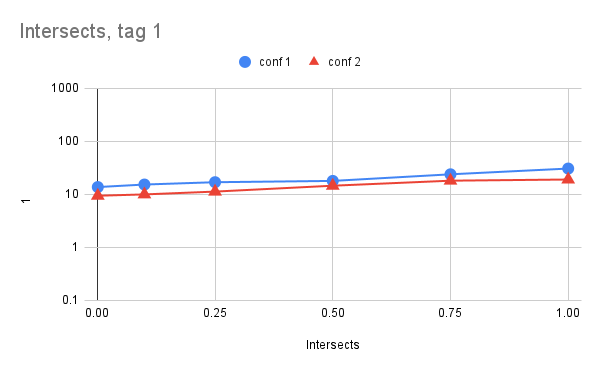
\includegraphics[width=\linewidth]{img/Intersects-tag-1.png}
    \caption{Syntetic workload, intersects, tag 1}\label{fig:intersects1}\par 
    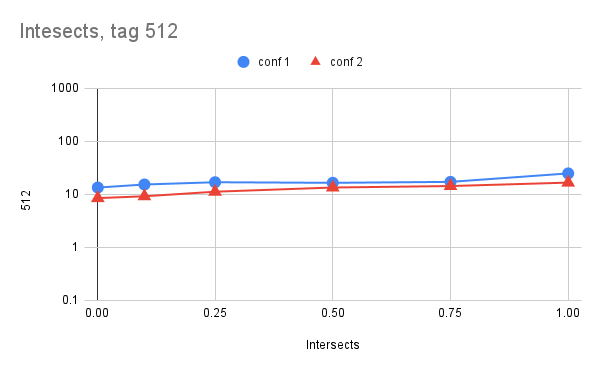
\includegraphics[width=\linewidth]{img/Intesects-tag-512.png}
    \caption{Syntetic workload, intersects, tag 512}\label{fig:intersects512}\par 
\end{multicols}
\begin{multicols}{2}
    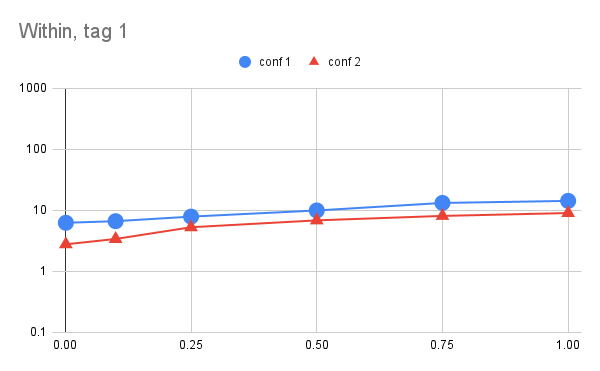
\includegraphics[width=\linewidth]{img/Within-tag-1.png}
    \caption{Syntetic workload, within, tag 1}\label{fig:within1}\par
    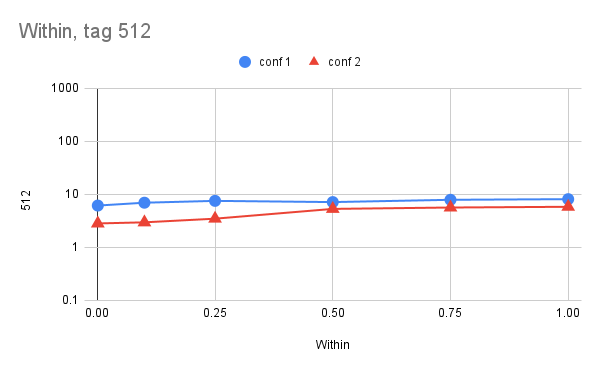
\includegraphics[width=\linewidth]{img/Within-tag-512.png}
    \caption{Syntetic workload, within, tag 512}\label{fig:within512}\par
\end{multicols}
\end{figure*}


The synthetic workload in Geographica 2 is designed using a generator that produces synthetic datasets of varying sizes, enabling the controlled evaluation of geospatial triplestores. This generator not only creates datasets with specific characteristics but also instantiates query templates that vary in both thematic and spatial selectivity. By doing so, Geographica 2 allows for a systematic examination of performance under different data and query conditions, from highly selective spatial queries to more comprehensive queries with minimal selectivity. 

This synthetic workload approach enables precise and repeatable performance assessments, ensuring that the evaluation of geospatial triplestores is not influenced by unpredictable real-world data variations. Through this controlled environment, researchers can measure the efficiency, scalability, and responsiveness of geospatial stores across a range of scenarios. This setup is invaluable for identifying performance trends and limitations that may be obscured in real-world datasets, making it possible to optimize triplestore configurations based on specific workload demands.

The \Cref{fig:intersects1,fig:intersects512,fig:within1,fig:within512} presented in this section illustrate response times for two configurations of GeoSPARQL Fuseki (conf 1 and conf 2) under various intersect and within conditions, where these configurations differ in their optimization settings. Analyzing the results, we observe a consistent trend where response times are influenced by both the proportion of matching features and the THEMA parameter value, with configuration 2 consistently outperforming configuration 1 across most cases.

For the `Intersects` predicate with THEMA set to 1, configuration 2 demonstrates superior efficiency, particularly as the query becomes more selective (e.g., filtering down to 0.01\% of the dataset features). This configuration shows a marked reduction in response time as the query specificity increases, reaching as low as 9.42 seconds for the most selective queries. This suggests that configuration 2 has optimizations that particularly benefit sparse spatial query results. In contrast, configuration 1, while generally slower, maintains steady performance across larger subsets (e.g., 50\% or more of dataset features), indicating its relative robustness in handling higher data loads.

When examining `Intersects` with THEMA set to 512, we observe similar patterns. Configuration 2 again outpaces configuration 1, achieving a response time as low as 8.5 seconds for the most selective cases (0.01\% of features). Notably, both configurations display a slight increase in response time when selecting 75\% or more of the dataset features, though configuration 2 remains more efficient under all proportions tested.

The `Within` predicate results show an even more pronounced efficiency for configuration 2. With THEMA at 1, configuration 2 achieves response times as low as 2.78 seconds for highly selective queries (0.01\% of features), a substantial improvement over configuration 1. For the `Within` predicate with THEMA set to 512, configuration 2 maintains similar advantages, particularly in selective queries, reaching response times as low as 2.83 seconds. Configuration 1 shows relatively steady performance here, but the times are consistently higher than those of configuration 2.

Overall, the data suggests that configuration 2 is well-suited for scenarios where high selectivity in spatial data queries is required, demonstrating reduced response times even in cases involving small feature subsets. In contrast, configuration 1 performs adequately in scenarios with broader data requirements, providing steady response times but lagging in more selective tasks. These findings highlight the flexibility and efficiency of GeoSPARQL Fuseki’s configurations in handling varied spatial query demands, emphasizing configuration 2’s advantage in optimized query processing for sparse result sets.

When comparing Fuseki's performance in the synthetic workload with its performance in real-world datasets, a clear trend emerges: the query response times in the synthetic workload exhibit a linear behavior within the range of $10^1$ seconds. This consistency across query types and dataset sizes suggests that Fuseki's optimizations are particularly effective under controlled conditions, as demonstrated in the synthetic workload generated by Geographica 2. 

In this context, Fuseki’s linear performance highlights its stability and scalability for geospatial queries, maintaining predictable response times even as the volume of queried features increases. The synthetic dataset’s controlled environment, with varying degrees of thematic and spatial selectivity, allows Fuseki to leverage indexing and optimization mechanisms effectively, thereby producing linear performance trends. In contrast, real-world datasets, with their inherent variability and less predictable distributions of geospatial features, may challenge triplestore optimizations in ways that deviate from this linear trend. 

This comparison underscores the efficiency of Fuseki in handling synthetic data, where controlled conditions allow it to deliver response times within a narrow and predictable range. Such performance insights are crucial for understanding Fuseki’s potential scalability and adaptability in varied environments and emphasize the importance of optimization in achieving consistent query response times across diverse geospatial workloads.


\section{Querying and Visualization}\label{VI-sec:querying}
The \textit{Querying} module serves as the final component of the framework, designed to facilitate user interaction with the knowledge graph, thereby transforming it into a dynamic, interactive tool for data exploration and analysis. This module offers sophisticated querying capabilities, particularly well-suited for handling complex geospatial data, and enables users to derive meaningful insights by directly engaging with the structure and content of the knowledge graph.


\subsection{Querying}\label{VI-subsec:querying}

At the core of this module’s functionality lies its proficient utilization of \acrshort{SPARQLLabel} \cite{ericprudhommeauxSPARQLQueryLanguage2008} and its querying capabilities, empowering users to execute complex queries that leverage geospatial relationships and extract data based on specific criteria. The module facilitates queries that traverse and interpret the rich semantic and geographic interconnections embedded in the knowledge graph. For instance, users can specify queries to retrieve all farms situated within a given radius of a water source or to identify regions contiguous to a particular city. These examples illustrate the ability to integrate both spatial and relational data, enabling the exploration of intricate geographic and topological relationships across varied datasets.

Moreover, the module extends beyond conventional querying by incorporating advanced geospatial functions through GeoSPARQL \cite{matthewperryOGCGeoSPARQLGeographic2012}. This integration empowers users to formulate spatial queries grounded in geographic features, such as exact coordinates or relative proximity to specified landmarks. By defining queries with detailed spatial parameters, users can enhance data retrieval processes to align with precise geospatial criteria. This capacity significantly broadens analytical possibilities, addressing questions that require a sophisticated understanding of spatial distribution, adjacency, and other complex geographic patterns.

Through the interplay of these functionalities, the Querying module offers a holistic and dynamic means of interacting with the knowledge graph. It provides a robust mechanism for \acrshort{SPARQLLabel}-based data retrieval while seamlessly integrating geospatial parameters and GeoSPARQL-driven queries, facilitating a multidimensional exploration of both relational and spatial aspects of the data. Consequently, the module transforms the knowledge graph into a powerful instrument for analyzing geospatial information, fostering deeper engagement and enabling a comprehensive exploration of geographic and topological insights.


\subsection{Visualization}\label{VI-subsec:visualization}

\subsubsection{Story Maps}

The visualization module in the framework utilizes the \acrfull{SMBVTLabel} module to render graphs as Story Maps, a concept introduced in \cite{bartalesiWebToolCreate2023c, bartalesiUnstructuredTextsSemantic2023b}. Story Maps are a visualization paradigm focused on presenting maps as dynamic narratives, where sequences of events are enriched with multimedia elements to create an engaging, spatially structured storytelling experience. Many software solutions exist for creating and visualizing story maps, with a focus on platforms that enable users to integrate text, images, audio, and video. These platforms aim to produce interactive, map-based narratives that guide users through immersive storytelling paths.

ArcGIS StoryMap is one of the foremost platforms in this area, known for its flexibility in designing, publishing, and sharing interactive story maps \cite{walsheUsingArcGISOnline2016}. This software allows for a high degree of customization, permitting users to augment their narrative flow through the incorporation of diverse multimedia elements. Although ArcGIS StoryMap offers an array of commercial versions with expanded features, a free version is also available. However, the free version comes with several restrictions: it lacks support for embedding external web pages, limits advanced map interaction capabilities, and reduces options for theme customization. Accessibility settings are similarly constrained, and perhaps most notably, the free version does not support integration with entities from existing knowledge bases such as Wikidata.\footnote{These limitations in the free version reflect typical restrictions in proprietary storytelling platforms, which may constrain the degree of interactivity and linkage to external datasets.}

In contrast, Timescape is another map-based storytelling tool that allows users to enrich events with text, images, and external links \cite{Timescape}. Like ArcGIS, Timescape is a commercial product, although a free tier allows for the creation of up to five story maps. A distinctly different tool, StoryMapJS, offers a fully free option accessible online or as a JavaScript library \cite{knightlabStoryMapJS}. StoryMapJS organizes stories through a sequence of slides, each depicting an event tied to a specific location, and enables users to link multimedia content to these events. By leveraging Google accounts for editor access, StoryMapJS serves as a versatile tool for digital storytelling, albeit without some of the advanced customization options found in ArcGIS.

For users with web development experience, constructing story maps through custom HTML templates offers another viable method. An example is the Leaflet Storymaps template, which guides readers through a point-by-point narrative while integrating scrolling features to enhance engagement \cite{sveenAtlefrenStorymap2024}. This template provides options for embedding multimedia, such as images, audio, video, and scanned map backgrounds, with map data entered through connected Google Sheets or CSV files. The HTML template approach allows for a high degree of customization, though it requires a more significant initial setup and a greater technical proficiency.

Open-source tools like Odyssey.js present hybrid approaches to story map creation. Odyssey.js allows users to create story maps using Markdown, with a limited number of webpage templates to expedite the creation process \cite{Odysseyjs}. This combination of HTML coding and external data structuring provides some flexibility, although it requires a certain level of technical skill and may lack the seamless integration features found in more advanced platforms.

Despite their utility in building story maps, these tools exhibit significant limitations compared to the SMBVT module, particularly in their handling of semantic integration and story inter-linking. Unlike the software reviewed, SMBVT leverages Semantic Web technologies, enabling it to link seamlessly with structured knowledge bases like Wikidata, thereby supporting enhanced data integration and interconnectivity between stories. SMBVT’s fully free availability further distinguishes it by removing the access and functionality constraints often inherent in both commercial and open-source alternatives. This unique combination of semantic linking and accessibility establishes SMBVT as an innovative tool in the field of story map creation, effectively addressing the common drawbacks of existing platforms and equipping users with a powerful solution for creating semantically enriched story maps.

\subsubsection{Other Visualization}

While Story Maps provide a compelling narrative-driven approach to visualizing data, there are alternative methods that offer distinct advantages for enhancing the usability and adaptability of NOnt+S across various contexts. Exploring these alternatives reveals opportunities to complement Story Maps, catering to diverse user needs and scenarios.

One approach involves the use of timelines, which emphasize temporal data by presenting sequential events in a linear or interactive format. This method enables users to explore historical developments, project schedules, or event sequences effectively. Similar to Story Maps, timelines can be enriched with multimedia elements, but their primary focus is on temporal progression rather than spatial narratives. This makes them particularly well-suited for applications where chronology is more significant than location. Furthermore, the temporal dimension highlighted in timelines can be integrated into Story Maps, providing a comprehensive view that combines both spatial and chronological contexts.

Network graphs offer another complementary visualization method, emphasizing relationships and connections within datasets. By visualizing entities as nodes and their interactions as edges, network graphs are particularly effective in fields like social network analysis, citation mapping, and knowledge graph representation. Their ability to reveal complex interdependencies and patterns makes them a powerful tool for representing semantic structures and linking narratives in NOnt+S, augmenting the capabilities of Story Maps.

Immersive 3D visualizations, such as virtual reality (VR) and augmented reality (AR), provide an experiential dimension to data visualization. These technologies enable users to navigate spatially complex datasets in simulated environments, enhancing spatial awareness and engagement. Applications range from urban planning and archaeology to scientific simulations, where spatial context and interaction are integral to understanding.


Lastly, heatmaps and geospatial analytics complement map-based storytelling by providing high-level overviews of data distributions and trends. These visualizations excel in scenarios requiring aggregated insights, such as demographic studies, environmental monitoring, and public health analyses. Their ability to convey density and intensity in spatial contexts adds depth to the insights derived from Story Maps, offering alternative perspectives on the same data.

By integrating these visualization approaches, NOnt+S can expand its usability across varied contexts. Interactive dashboards promote data-driven exploration; network graphs elucidate relationships; immersive 3D visualizations enhance experiential engagement; timelines provide temporal clarity; and heatmaps enable high-level spatial analysis. Together, these methods enrich the visualization landscape, ensuring that NOnt+S adapts seamlessly to the needs of diverse audiences and applications.


% \section{Integration of Case Studies}

% The framework has been applied to datasets from the \textit{MOVING} and \textit{IMAGO} projects, each of which provided unique challenges for geospatial data representation and reasoning. Through the framework, these datasets were transformed into enriched knowledge graphs that support advanced geospatial queries and reasoning.

% For the \textit{MOVING} project, the framework handled agricultural data, such as farm locations, crop yields, and environmental factors. The \textit{IMAGO} project, on the other hand, dealt with geographic narratives, requiring the framework to capture complex spatial relationships between historical events and geographic features.


\section{Scalability and Generalizability of the Framework}\label{VI-sec:scalability}

The NOnt+S framework is built with scalability and generalizability as foundational principles, enabling it to adapt to varying data sizes, complexities, and application contexts. Scalability is achieved through its modular architecture, which allows independent components such as data linking, semantic enrichment, and reasoning to operate efficiently even as data volumes increase. For example, the triplestore, central to data storage and querying, can be expanded using distributed systems or cloud-based infrastructures. By integrating efficient reasoning engines like Openllet, the framework ensures that computational demands are kept manageable, even when processing extensive datasets.

Performance testing, particularly with synthetic datasets under the Geographica 2 benchmark, has demonstrated the framework’s capability to maintain linear query response times even as dataset sizes grow significantly. This ensures that the system remains responsive and efficient, making it suitable for both small-scale applications and those involving massive geospatial data repositories.

The framework’s generalizability lies in its ability to adapt to a broad range of domains and datasets. While the NOnt+S ontology forms its semantic backbone, the architecture supports the integration of alternative ontologies tailored to specific fields. Its compatibility with diverse data sources such as Wikidata, GeoNames, and OpenStreetMap underscores its flexibility in handling varied schemas and granularities. This adaptability has been validated through its application to case studies in agricultural and historical narratives, showcasing its potential across disciplines like urban planning, cultural heritage, and environmental science.

By adhering to established standards such as RDF, OWL, and SPARQL, the framework ensures interoperability with other semantic systems and tools. This alignment not only broadens its utility but also facilitates seamless data sharing and integration. Moreover, its querying and visualization capabilities, including the ability to construct dynamic Story Maps and other visual representations, provide users with versatile tools to explore and communicate insights.

Despite its strengths, challenges remain in addressing real-time data integration, optimizing usability for non-experts, and ensuring efficiency in resource-constrained environments. For instance, incorporating IoT sensor data or handling dynamic geospatial changes would require further optimization of data ingestion and reasoning processes. Enhancing the user interface to simplify the construction of complex queries would also help democratize its usage, particularly for non-technical users.


\section{Conclusion}

The architecture of the NOnt+S evaluation framework provides a robust, modular system for processing, analyzing, and visualizing geospatial data. By integrating modules for linking, representation, reasoning, storage, and querying, the framework enables the creation of a dynamic geospatial knowledge graph. This architecture supports interdisciplinary research, providing valuable insights into both agricultural and geographic domains through its advanced semantic capabilities.
